\documentclass{standalone}
\usepackage{tikz}
\usepackage{tikz-3dplot}
%%%<


%% document-wide tikz options and styles
\begin{document}
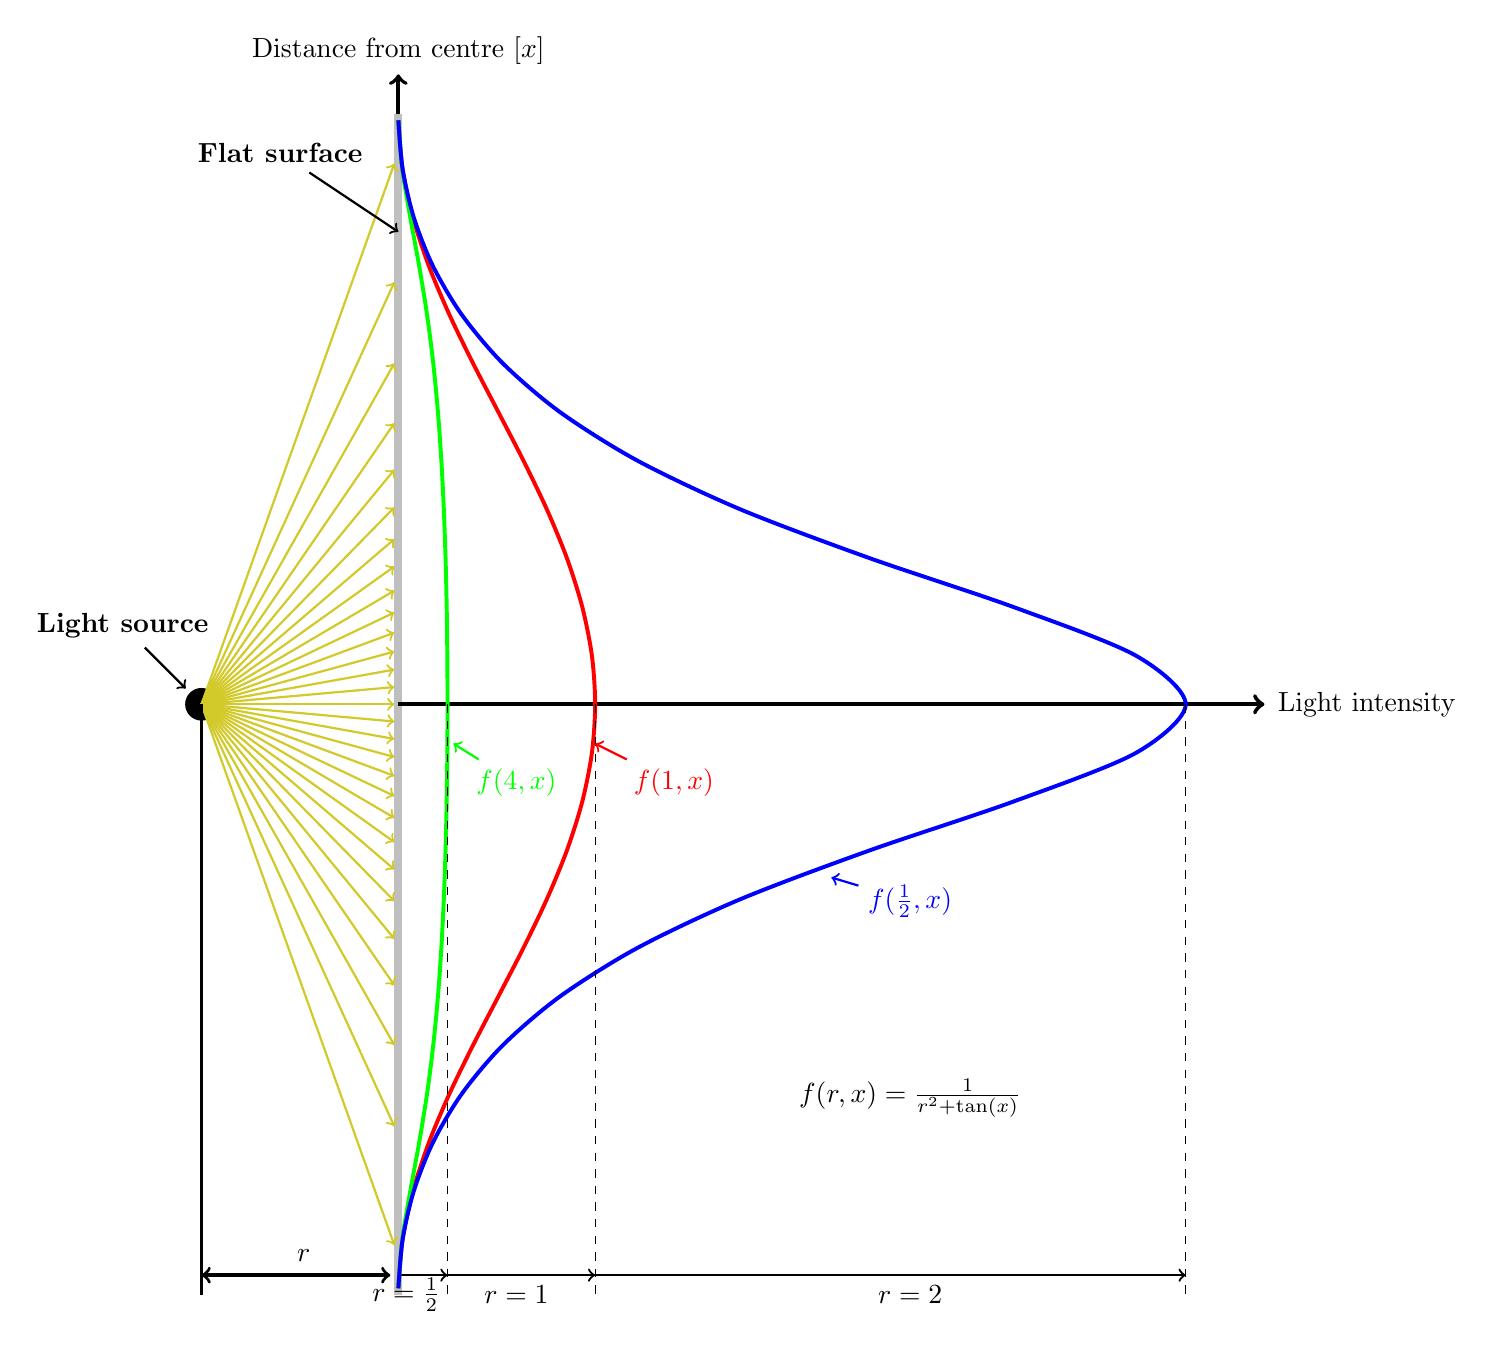
\begin{tikzpicture}

\begin{scope}[scale=0.5]
  \draw[line width=1mm, lightgray](5,-15)--(5,15);
\draw[fill = black](0,0) circle(0.4);
\foreach \i in {-70,-65,...,70}
{
	\draw[thick,->,yellow!80!black](0,0)--(4.9,{5*tan(\i)});
}
%\draw[ultra thick,->,yellow!80!black](0,0)--(5,{5*tan(10)});
\draw[thick](0,0)--(0,-15);
\draw[<->,very thick](0,-14.5)--(4.8,-14.5);

\draw[->,ultra thick](5,0)--(27,0);
\draw[->,thick](5,-14.5)--({(10+10/(4))/2},-14.5);
\draw[->,thick](5,-14.5)--({(10+10/(1))/2},-14.5);
\draw[->,thick](5,-14.5)--({(10+10/(0.25))/2},-14.5);
 
 %\draw[line width=2mm, gray](5.1,-10)--(5.1,10);
 
 \draw[line width=0.5mm,scale=0.5,domain=-89:89,smooth,variable=\y,red]  plot ({10+10/(1+tan(\y)^2)},{\y/3});
 
  \draw[line width=0.5mm,scale=0.5,domain=-89:89,smooth,variable=\y,green]  plot ({10+10/(4+tan(\y)^2)},{\y/3});
  \draw[line width=0.5mm,scale=0.5,domain=-89:89,smooth,variable=\y,blue]  plot ({10+10/(0.25+tan(\y)^2)},{\y/3});
  \draw[->,line width=0.5mm](5,15)--(5,16);
  \draw[dashed]({(10+10/(4))/2},0)--({(10+10/(4))/2},-15);
  \draw[dashed]({(10+10/(1))/2},0)--({(10+10/(1))/2},-15);
  \draw[dashed]({(10+10/(0.25))/2},0)--({(10+10/(0.25))/2},-15);
 \end{scope}
 
 
 \node[fill=white](stxt) at (-1,1){\textbf{Light source}};
 \draw[->,thick](stxt)--(-0.2,0.2);
 \node[fill=white](stxt) at (1,7){\textbf{Flat surface}};
 \draw[->,thick](stxt)--(2.5,6);
 
  \node[very thick,fill=white] at (1.3,-7){\textbf{$r$}};
  \node[] at (2.6,-7.5){\textbf{$r=\frac{1}{2}$}};
  \node[fill=white] at (4,-7.5){\textbf{$r=1$}};
  \node[fill=white] at (9,-7.5){\textbf{$r=2$}};
  \node[fill=white] at (9,-5){$f(r,x)=\frac{1}{r^2+\tan(x)}$};
  \node[blue](bla) at (9,-2.5){$f(\frac{1}{2},x)$};
  \draw[->,thick,blue](bla)--(8,-2.2);
  \node[red](re) at (6,-1){$f(1,x)$};
  \draw[->,thick,red](re)--(5,-0.5);
  \node[green](gre) at (4,-1){$f(4,x)$};
  \draw[->,thick,green](gre)--(3.2,-0.5);
  
  \node[]at (14.8,0){Light intensity};
  \node[]at (2.5,8.3){Distance from centre $[x]$};
\end{tikzpicture}
\end{document}
